% \documentclass[aspectratio=169,notes]{beamer}
\documentclass[aspectratio=169]{beamer}
\usetheme[faculty=phil]{fibeamer}
\usepackage{polyglossia}
\setmainlanguage{english} %% main locale instead of `english`, you
%% can typeset the presentation in either Czech or Slovak,
%% respectively.
\setotherlanguages{russian} %% The additional keys allow
%%
%%   \begin{otherlanguage}{czech}   ... \end{otherlanguage}
%%   \begin{otherlanguage}{slovak}  ... \end{otherlanguage}
%%
%% These macros specify information about the presentation
\title[Theoretical Mechanics]{Big HW 2} %% that will be typeset on the
\subtitle{ Dynamics \\
\  \\ \  \
         } %% title page.
\author{Oleg Bulichev}
%% These additional packages are used within the document:
\usepackage{ragged2e}  % `\justifying` text
\usepackage{booktabs}  % Tables
\usepackage{tabularx}
\usepackage{tikz}      % Diagrams
\usetikzlibrary{calc, shapes, backgrounds}
\usepackage{amsmath, amssymb}
\usepackage{url}       % `\url`s
\usepackage{listings}  % Code listings
% \usepackage{subfigure}
\usepackage{floatrow}
\usepackage{subcaption}
\usepackage{mathtools}
\usepackage{todonotes}
\usepackage{fontspec}
\usepackage{multicol}
\usepackage{pdfpages}
\usepackage{wrapfig}
\usepackage{animate}
\usepackage{booktabs}
\usepackage{multirow}
% \usepackage{graphicx}
\usepackage{colortbl}

\graphicspath{{resources/}}
\frenchspacing

\setbeamertemplate{caption}[numbered]
\usetikzlibrary{graphs}

% \usepackage[backend=biber,style=ieee,autocite=footnote]{biblatex}
% \addbibresource{biblio.bib}
% \DefineBibliographyStrings{english}{%
%   bibliography = {References},}

\newcommand{\oleg}[2][] {\todo[color=red, #1] {OLEG:\\ #2}}
\newcommand{\fbckg}[1]{\usebackgroundtemplate{\includegraphics[width=\paperwidth]{#1}}}%frame background

\usepackage[framemethod=TikZ]{mdframed}
\newcommand{\dbox}[1]{
\begin{mdframed}[roundcorner=3pt, backgroundcolor=yellow, linewidth=0]
\vspace{1mm}
{#1}
\vspace{1mm}
\end{mdframed}
}

\begin{document}
\setlength{\abovedisplayskip}{0pt}
\setlength{\belowdisplayskip}{0pt}
\setlength{\abovedisplayshortskip}{0pt}
\setlength{\belowdisplayshortskip}{0pt}

\fbckg{fibeamer/figs/title_page.png}
\frame[c]{\setcounter{framenumber}{0}
    \usebeamerfont{title}%
    \usebeamercolor[fg]{title}%
    \begin{minipage}[b][6.5\baselineskip][b]{\textwidth}%
        \textcolor{black}{\raggedright\inserttitle}
    \end{minipage}
    % \vskip-1.5\baselineskip

    \usebeamerfont{subtitle}%
    \usebeamercolor[fg]{framesubtitle}%
    \begin{minipage}[b][3\baselineskip][b]{\textwidth}
        \raggedright%
        \insertsubtitle%
    \end{minipage}
    \vskip.25\baselineskip
}
%   \frame[c]{\maketitle}

\fbckg{fibeamer/figs/common.png}

\section*{Outline}
\begin{frame}[t]{Outline}
\framesubtitle{}
\tableofcontents
\end{frame}

\section{General ideas beside HW}
\begin{frame}[t]{General ideas beside HW}
\framesubtitle{}
\vspace{-0.4cm}
  \begin{itemize}
    \item It is a research homework, hence there is no unique right answer. Therefore, you have to prove your solution.
    \item The report should be unique, but you can do it in groups. But you must record who did what. Like, <<Katya gathered a dataset, Ahmed measured a stand>> and so on.
    \item You can read papers, use solutions from the internet, that's fine. But you have to mention it in the report.
  \end{itemize}
\end{frame}

\section{Global task description}
\begin{frame}[t]{Global task description}
  \vspace{-0.4cm}
\framesubtitle{}
      There is the cart pole system in the lab. Your global goal is to create a math model of it and prove that the model is really describes it.
      \medskip

      \begin{figure}[H]
        \centering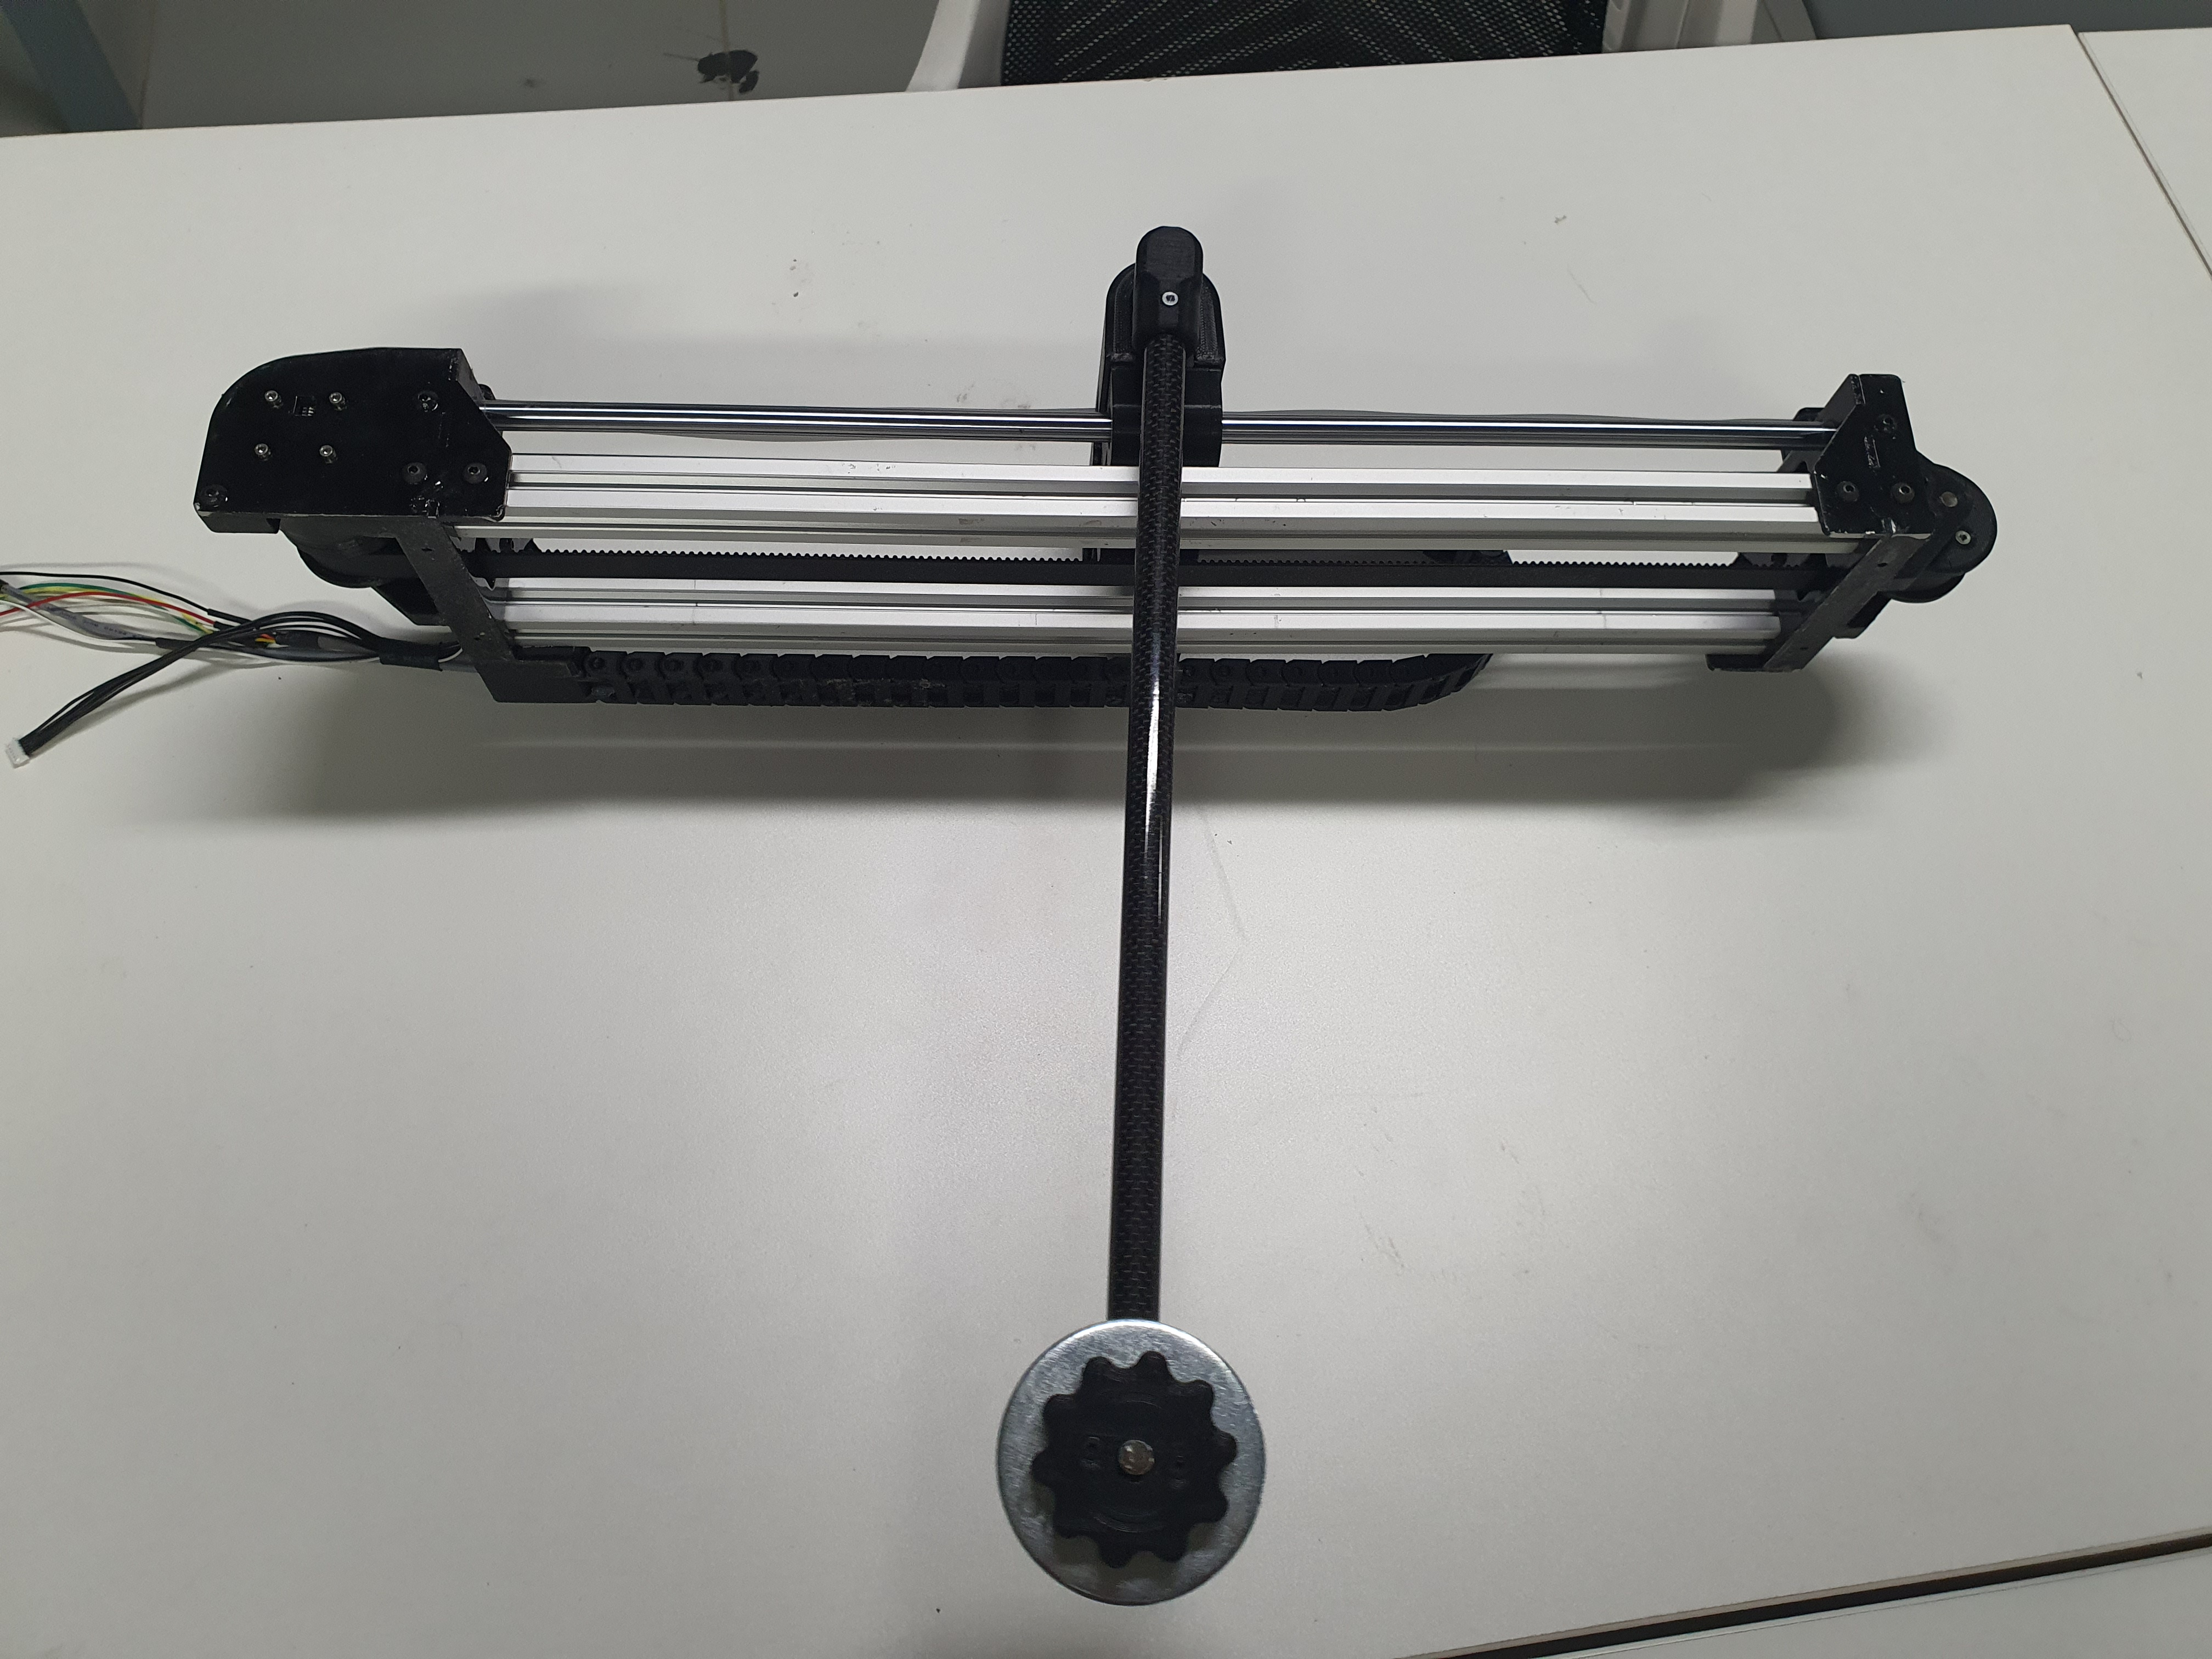
\includegraphics[height=4cm,width=1\textwidth,keepaspectratio]{experimental_stand.JPG}
        \caption*{Cart pole in the dungeon}
        \label{fig:experimental_stand.JPG}
      \end{figure}
\end{frame}


\section{Detailed task description}
\begin{frame}[t]{Detailed task description}
\framesubtitle{}
\vspace{-0.4cm}
\footnotesize
\begin{enumerate}
  \item Obtain the required measurements of the stand (like needed masses, lengths and so on).
  \item Gather the positions and velocities of the stand. You should run the same experiment 3 times each. 
  
  Initial conditions:
  \begin{itemize}
    \footnotesize
    \item $x = 0,\ \phi = 15^\circ,\ \dot{x} = 0,\ \dot{\phi} = 0,\ t=0$;
    \item $x = 0.25\ m,\ \phi = 45^\circ,\ \dot{x} = 0,\ \dot{\phi} = 0,\ t=0$;
    \item $x = 0.25\ m,\ \phi = -135^\circ,\ \dot{x} = 0,\ \dot{\phi} = 0,\ t=0$;
  \end{itemize}
  \item Substitute a real data to your math model from HW 7, 8 (you can choose any method your like) and compare the results (propose and justify the metric).
  \item Explain, what affects the difference between math model and real data. Is it difference significant? 
  \item If so, change the model (add new forces, change the object representation), gather new needed data and compare it again.
  \item Make a conclusion.
\end{enumerate}
\end{frame}

\section{What report should contain}
\begin{frame}[t]{What report should contain}
\framesubtitle{}
\vspace{-0.4cm}
\begin{itemize}
  \item The list of used tools and applications (I gathered a trajectory dataset using $x$ tool), etc.
  \item The list of data you gathered from stand and how did you do it.
  \item Show how you conducted experiments. Is there any difference when you did the same experiment? Show it using plots and/or other metrics like $std,\ mse$ and so on.
  \item Show the way how you chose the metrics for trajectory comparison, how you justify the answer.
  \item If the error is too large, explain how you wanted to change your model and why you chose such path.
  \item Summarize your experience.
\end{itemize}
\end{frame}

\section{Hints}
\begin{frame}[t]{Hints}
\framesubtitle{}
\vspace{-0.4cm}
  \begin{itemize}
    \item To determine inertia, you can create (or find) a CAD model and take data from it, or you can do an actual experiment to determine it.
    \item When you perform the experiment, you can make a template (for example, a piece of paper with a 10-degree angle).
    \item For choosing a metric for how to compare trajectories, you can start with the concept of least squares.
    \item Some of the data for the math model can be taken from the stand itself (e.g., friction).
    \item Feel free to do a literature review to find good ideas. But you must show exactly what you used.
  \end{itemize}
\end{frame}

\fbckg{fibeamer/figs/last_page.png}
\frame[plain]{}
\end{document}